\documentclass[aspectratio=169,9pt]{beamer}

\usetheme[progressbar=frametitle]{metropolis}
\usepackage{appendixnumberbeamer}

\usepackage{booktabs}
\usepackage[scale=2]{ccicons}

\usepackage{pgfplots}
\usepgfplotslibrary{dateplot}

\usepackage{xspace}
\newcommand{\themename}{\textbf{\textsc{metropolis}}\xspace}

% Custom Tweaks
\setbeamercolor{background canvas}{bg=white}
\setbeamertemplate{caption}{\raggedright\insertcaption\par}

% -------------------------
% General Details for Title
% -------------------------
\title{JAMSTACK}
\author{Aromal Anil\\S7CS B}
\institute[College of Engineering Cherthala] 
{
\begin{small}
Guided By:\\Jisy Raju
\end{small}
\\Department of Computer Science and Engineering
}
\date{\today} 


% ------------------------
% Presentation Starts Here
% ------------------------
\begin{document}

% Title Page
\maketitle

% Overview Page
\begin{frame}{Overview}

    \begin{enumerate}
        \item History
        \item Introduction to Jamstack
        \item How Jamstack Works
\item Traditional Web vs Jamstack
        \item Why Jamstack
        \item Jamstack Concepts
        \item Tools for Jamstack
        \item Live Demo
        \item Reference
    \end{enumerate}
    
\end{frame}

%History Page
\section{History}
\begin{frame}{A Look Into The Past}

    \textbf{Problem with Legacy Web}
    \vspace{1em}
   \begin{itemize}
       \item For each request HTML page is generated in server.
       \item Backend focused, generally runs on a web server all the times.
       \item Backend \& Frontend are coupled together.
       \item Provides way too many opportunities for attack.
       \item Expensive to scale.
   \end{itemize}

\end{frame}

\begin{frame}{Static Websites vs Dynamic Websites}
\vspace{2em}
\begin{columns}
\centering
\begin{column}{0.47\textwidth}
        \textbf{Static Websites}
        \vspace{1em}
        \begin{itemize}
%         \setlength{\itemsep}{.8em}
            \item It sends exactly the same response for every request.
            \item Will not contain dynamic data.
            \item Content changes only when someone publishes and updates the file.
        \end{itemize}
    \end{column}
    \begin{column}{0.47\textwidth}
       \textbf{ Dynamic Websites}
       \vspace{1em}
        \begin{itemize}
%         \setlength{\itemsep}{.8em}
            \item It may generate different HTML for each of the request.
            \item Can contain dynamic data.
            \item Server can generate unique content for each request using SSR.
        \end{itemize}
    \end{column}
\end{columns}
\vspace{1em}
    	\begin{figure}
        \begin{center}
            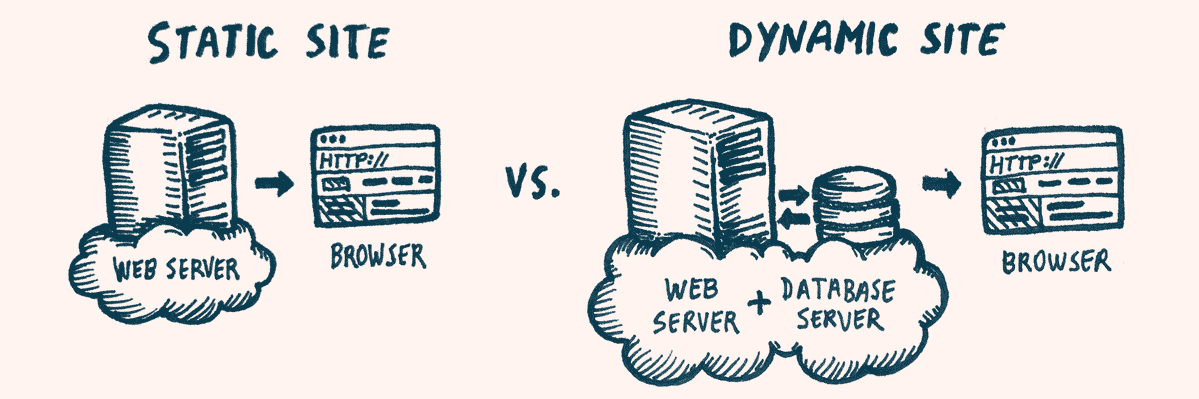
\includegraphics[scale=.25]{images/static-dynamic.png}
            \caption{Static vs Dynamic Websites ^{13}}
        \end{center} 
    \end{figure}
\end{frame}

\begin{frame}{Emerging of new Webstack}

    \textbf{What lead to the need for a new approach.}
    \vspace{1em}
    \begin{itemize}
       \item Static websites were not static anymore.
       \item Static website was able to show dynamic contents using JS \& AJAX calls.
       \item Emergence of modern frontend frameworks.
       \item Availability of backend features like routing in frontend.
       \item Introduction of Node.js, allowed JavaScript to work on the server-side.
       \item Introduction of Serverless functions.
       \item These arose the need for a frontend focused stack.
   \end{itemize}
\end{frame}

%What is Jamstack Page
\section{Introduction to Jamstack}
\begin{frame}{What is Jamstack}
    \begin{itemize}
        \item Stands for JavaScript, API & Markup.
        \item New approach to build fast and secure websites.
        \item Gives dynamic capabilities to static websites.
    \end{itemize}
    
    \vfill
    
    \begin{figure}
        \begin{center}
            
\includegraphics[scale=.18]{./images/components.png}
            \caption{Components of Jamstack ^1}
        \end{center} 
    \end{figure}
    
\end{frame}

\begin{frame}{JavaScript}
\begin{figure}
        \begin{center}
            
\includegraphics[scale=.15]{./images/javascript.png}
            \caption{JavaScript ^2}
        \end{center} 
    \end{figure}
\begin{itemize}
    \item Adds dynamic interactions to the website.
    \item Make client side rendering possible.
    \item No restriction on libraries/ frameworks you must use.
\end{itemize} 
\end{frame}

\begin{frame}{API}
\begin{figure}
        \begin{center}
            
\includegraphics[scale=.16]{./images/api.png}
            \caption{API ^3}
        \end{center} 
    \end{figure}
\begin{itemize}
    \item Server side operations are abstracted into APIs.
    \item Accessed using JavaScript over HTTP/HTTPS.
    \item Each functions of sever can be split into separate APIs forming Microservices .
    \item Third party APIs could be used for adding functionality.
\end{itemize} 
\end{frame}

\begin{frame}{Markup}
    \begin{figure}
        \begin{center}
            
\includegraphics[scale=.15]{./images/html.png}
            \caption{Hyper Text Markup Language (HTML) ^4}
        \end{center} 
    \end{figure}
\begin{itemize}
    \item Any form of markup language like HTML, Markdown etc.
    \item During build process other forms of markups are converted into HTML pages.
    \item Static site generators can generate static HTML using data from database & markup file.
\end{itemize} 
\end{frame}


\section{How Jamstack Works}

\begin{frame}{How Jamstack Works}
    \begin{itemize}
    \setlength{\itemsep}{.8em}
        \item Static files are generated during development or build process.
        \item Pre-built markup and assets are served to user on request.
        \item Browser executes JavaScript after HTML page is loaded.
        \item For any dynamic functionalities API call is done.
        \item The JavaScript updates the page according to the response from the API.
    \end{itemize}
    
\end{frame}

\begin{frame}{Static Site Generators}
\vspace{2em}
\begin{itemize}
    \item Takes Markup/Template/Data \& convert it into web pages during build process.
    \item Since web pages are generated during build time, it eliminates the need to render pages on request.
\end{itemize}
\vfill
\begin{figure}
        \begin{center}
            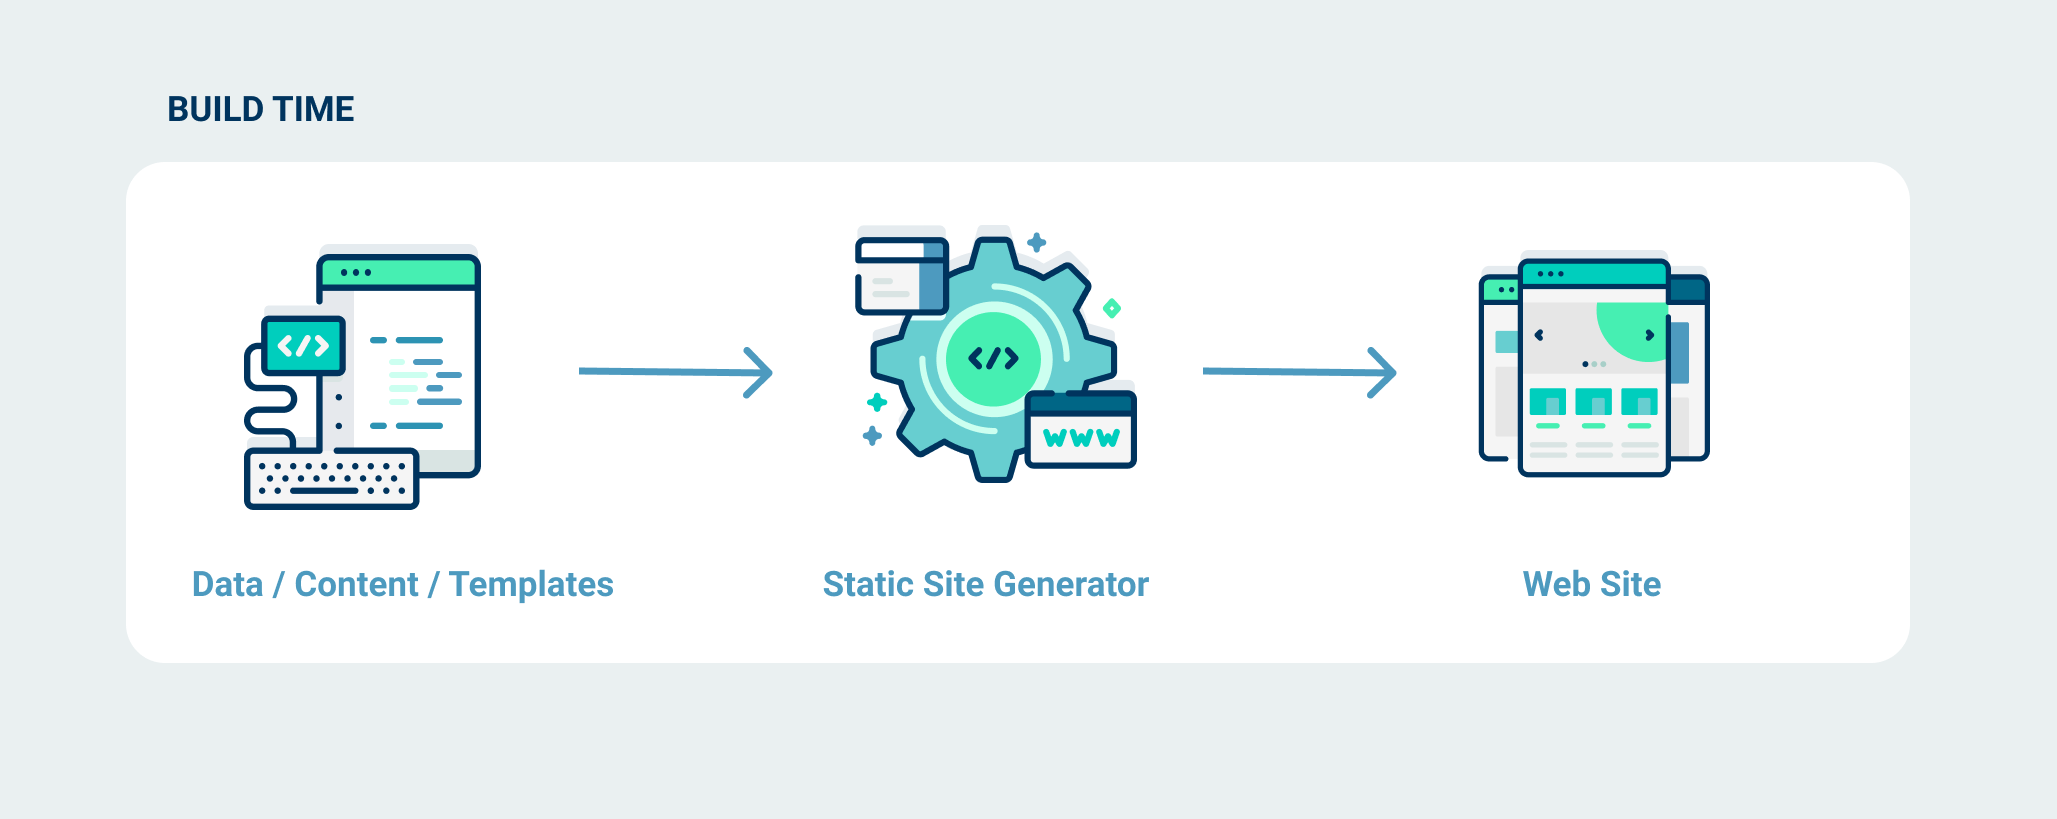
\includegraphics[scale=.12]{images/static-site-generators.png}
            \caption{Working of Static Site Generators ^{12}}
        \end{center} 
\end{figure}
    
\end{frame}

\begin{frame}{Jamstack Architecture.}
\vspace{2em}
\begin{figure}
    \begin{center}
            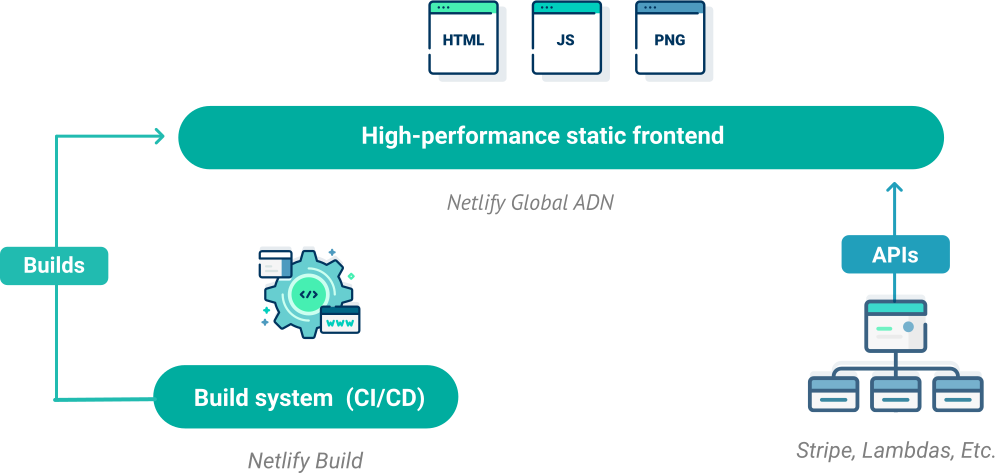
\includegraphics[scale=.3]{images/how-it-works.png}
            \caption{Jamstack Architecture ^5}
    \end{center}
    \end{figure}    
\end{frame}

\section{Traditional Web vs Jamstack}
\begin{frame}{Traditional Web vs Jamstack}

\begin{columns}
\centering
\begin{column}{0.47\textwidth}
        \textbf{Traditional Web}
        \vspace{1em}
        \begin{itemize}
        \setlength{\itemsep}{.8em}
  \item Frontend and Backend are \textit{Coupled}.
            \item Server side rendering.
            \item Content updates are pushed through traditional CMS, like WordPress or Drupal.
            \item Core updates pushed to server using FTP.
        \end{itemize}
    \end{column}
    \begin{column}{0.47\textwidth}
       \textbf{ Jamstack}
       \vspace{1em}
        \begin{itemize}
        \setlength{\itemsep}{.8em}
   \item Frontend and Backend are \textit{Decoupled}
            \item Webpages are pre-rendered.
            \item Content updates are pushed through Git or a headless CMS.
            \item Core updates are pushed through Git.
        \end{itemize}
    \end{column}
\end{columns}
    
\end{frame}

\begin{frame}{Traditional Web vs Jamstack}
\vspace{25pt}
\begin{figure}
    \begin{center}
        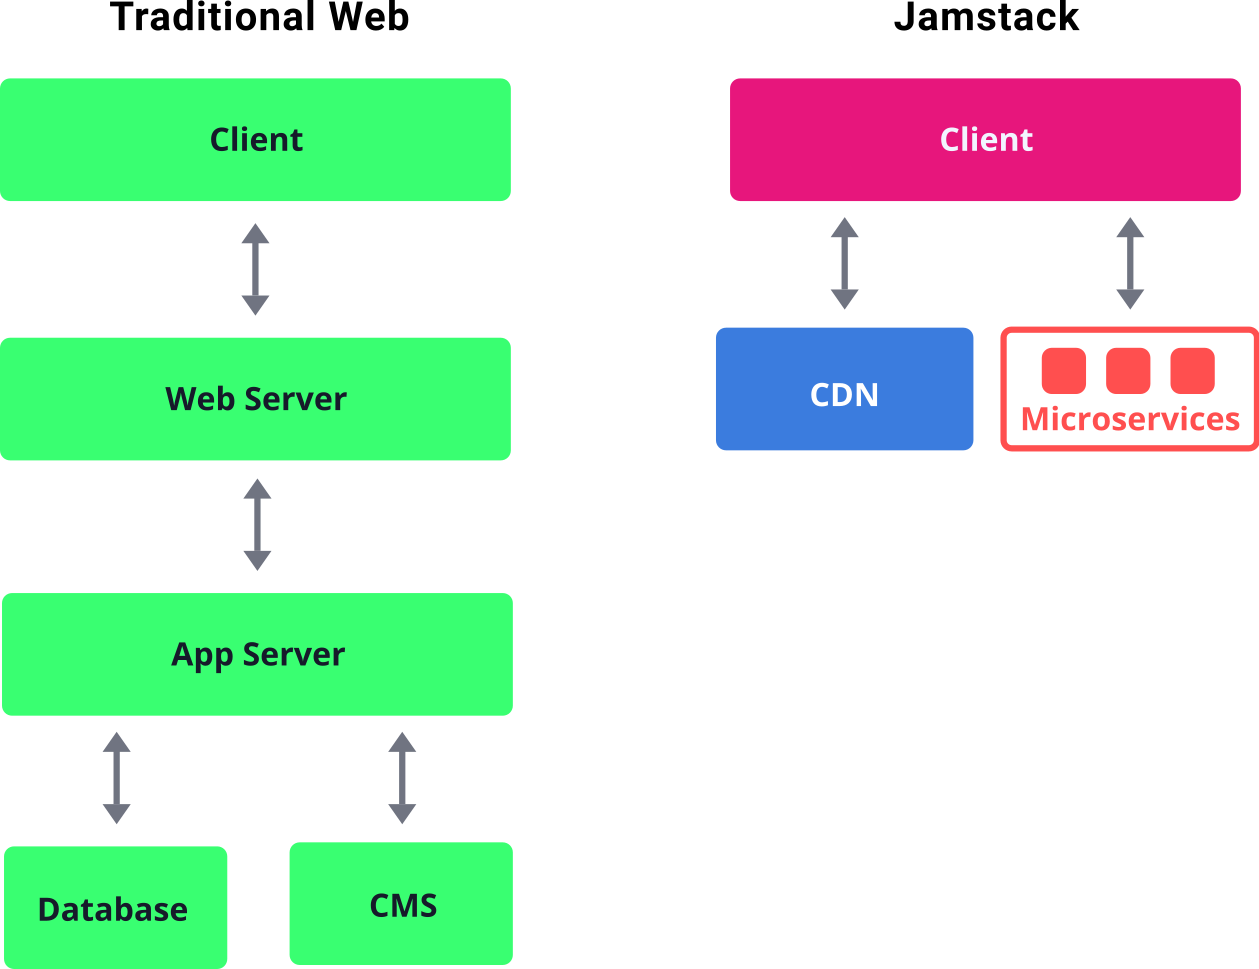
\includegraphics[scale=.68]{images/comparison.png}
        \caption{Traditional Web vs Jamstack ^6}
    \end{center}
\end{figure}
    
\end{frame}

\section{Why Jamstack ?}

\begin{frame}{What Makes Jamstack Great?}
    \vspace{2em}
    \begin{itemize}
        Jamstack apps inherently satisfy most of the 5 pillars of the \textbf{AWS Well-Architected Framework}.
    \end{itemize}
    \vfill
    \begin{figure}
        
\includegraphics[scale=.25]{images/aws-well-architected-framework.jpg}
        \caption{Characters of AWS well architected framework ^7}
    \end{figure}
    
\end{frame}

\begin{frame}{Fast Performance}
    \vspace{2em}
    \begin{itemize}
        \item Assets can be served as static files from a CDN.
        \item Server don't need to build the page on each request.
        \item Static content be reproduced and stored across the globe.
    \end{itemize}
    \vfill
    \begin{figure}
        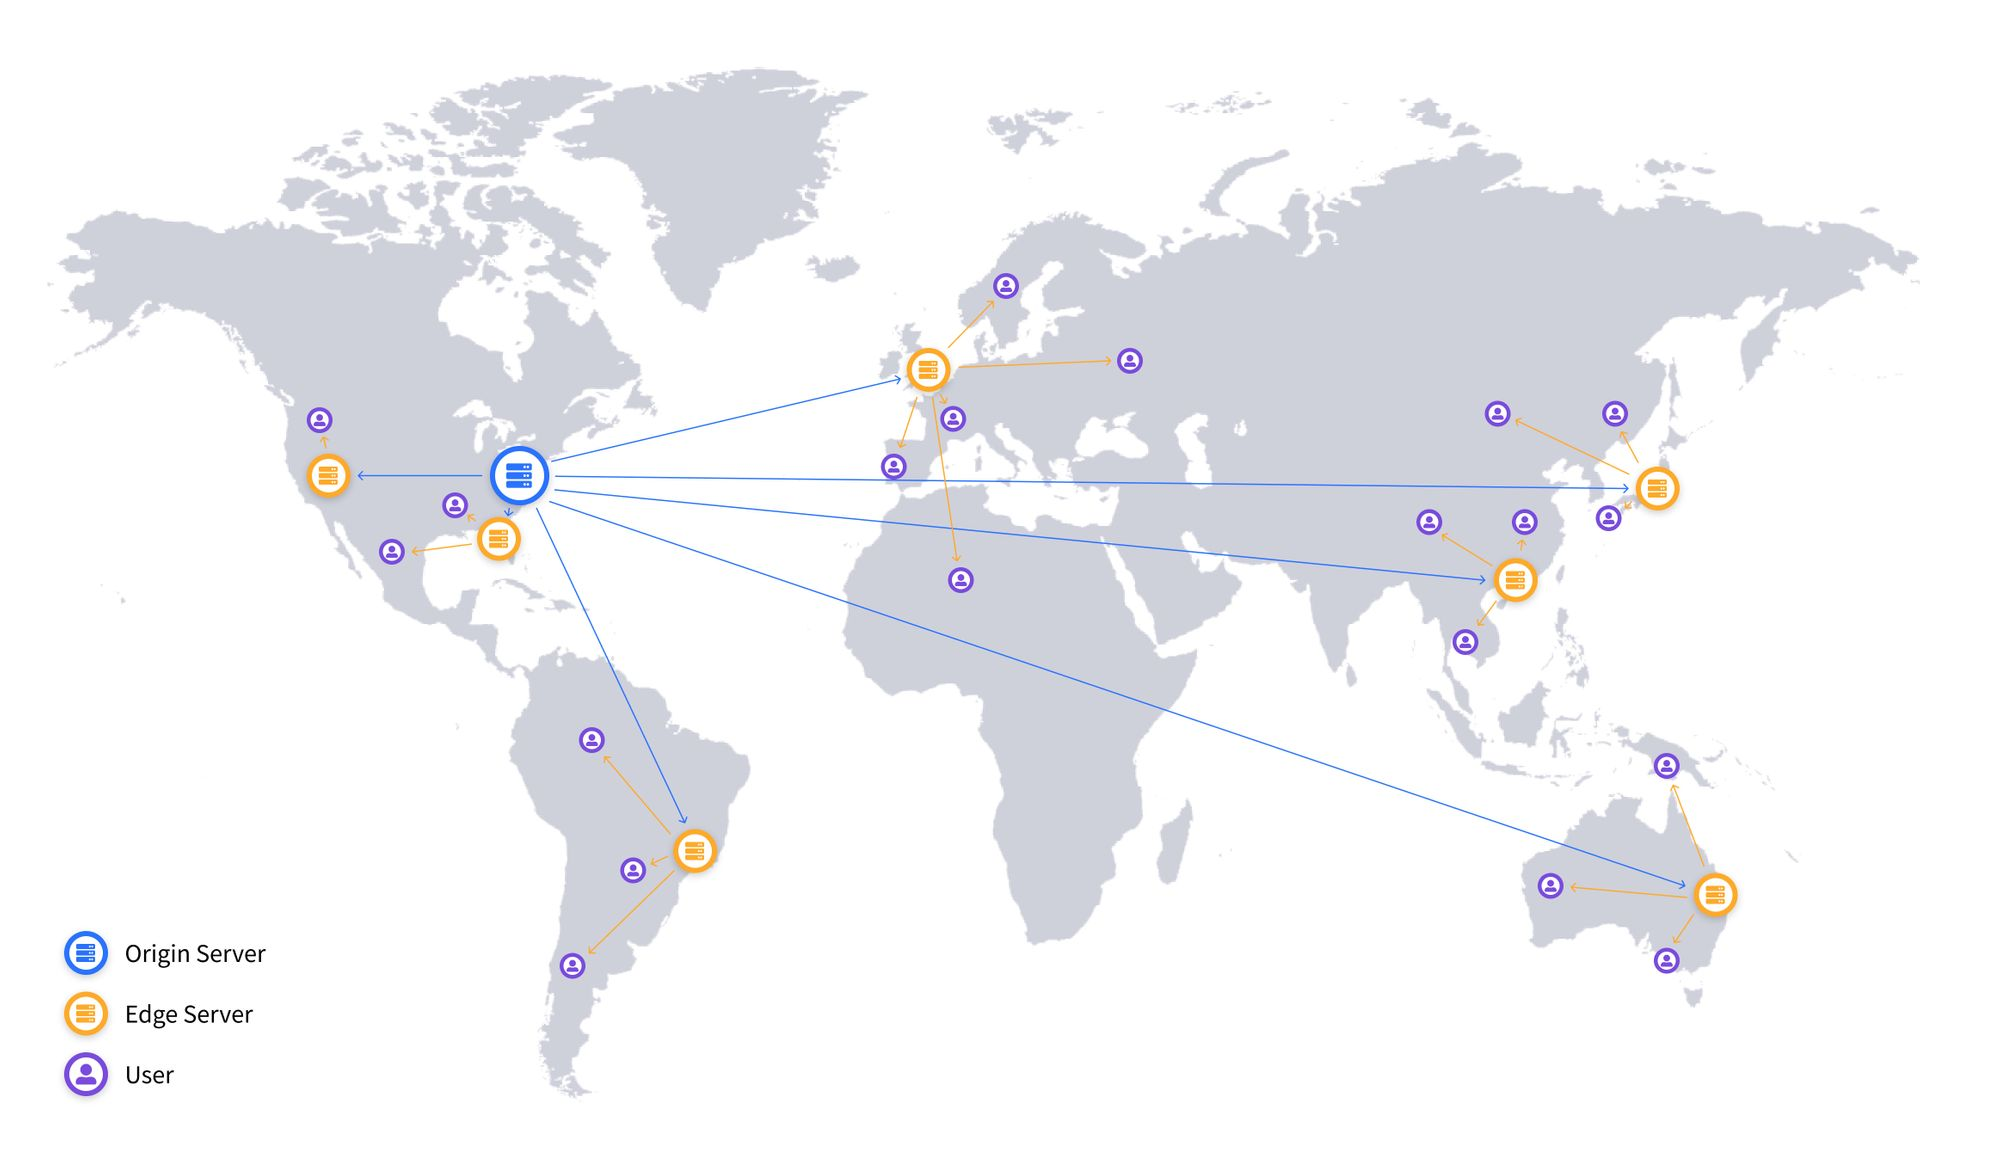
\includegraphics[scale=.1]{images/cdn-distribution-map.jpg}
        \caption{CDN Distribution map ^8}
    \end{figure}
\end{frame}

\begin{frame}{High security}
    \vspace{2em}
    \begin{itemize}
        \item Server-side logic is abstracted into APIs.
        \item User is served static HTML pages, without direct connection to the backend or database.
        \item Can use secure 3rd party APIs for specific needs like authentication.
    \end{itemize}
    \vfill
    \begin{figure}
        
\includegraphics[scale=.15]{images/apis.png}
        \caption{Available API Services ^9}
    \end{figure}
    
\end{frame}

\begin{frame}{Low cost}
    \vspace{2em}
    \begin{itemize}
        \item Static Assets can be cached in a CDN, which are generally cheap.
        \item Since SSR is not used, sever load is decreased.
        \item Use very few resources than alternatives.
    \end{itemize}
    \vfill
    \begin{figure}
        
\includegraphics[scale=.2]{images/netlify.png}
        \caption{Host Jamstack sites free on Netlify ^{10}}
    \end{figure}
    
\end{frame}

\begin{frame}{Better Developer Experience}
    \vspace{2em}
    \begin{itemize}
        \item No tight coupling between the application backend and frontend.
        \item Git based deployment makes deployment and development easy.
        \item Easy integration of third-party services like Algolia, Auth0, Cloudinary etc.
    \end{itemize}
    \vfill
    \begin{figure}
        
\includegraphics[scale=.13]{images/happy-developer.png}
        \caption{Happy Developers ^{11}}
    \end{figure}
    
\end{frame}

\section{Jamstack Concepts}
\begin{frame}{Concepts}
    \begin{itemize}
        \item \textbf{Decoupling} 
        \vspace{.5em}
        \begin{itemize}
        \setlength{\itemsep}{.4em}
            \item Separation of frontend pages and UI from the backend and databases.
            \item This separation allows frontend to be deployed separately
        \end{itemize}
        \vspace{1em}
        \item \textbf{Prebuilding}
        \vspace{.5em}
        \begin{itemize}
        \setlength{\itemsep}{.4em}
            \item Before deployment entire frontend is build into static pages and assets.
            \item Highly optimised.
            \item Example build step of a React app.
        \end{itemize}
        \vspace{1em}
        \item \textbf{Git Based Workflow}
        \vspace{.5em}
        \begin{itemize}
        \setlength{\itemsep}{.4em}
            \item Jamstack ties deployments closely to a Git-based workflows.
            \item Git brings the rigor and safety of version control to web projects.
            \item Allows support for numerous contributors with ease.
        \end{itemize}
    \end{itemize}
    
\end{frame}


\section{Tools for Jamstack}
\begin{frame}{Tools}

\begin{itemize}
    \item \textbf{Static Site Generators}
    \vspace{.5em}
    \begin{itemize}
    \setlength{\itemsep}{.4em}
        \item Generates static HTML and assets from Markdown or data fetched from database.
        \item Site Generation occurs during build time.
    \end{itemize}
    \vspace{1em}
    \item \textbf{Headless CMS}
    \vspace{.5em}
    \begin{itemize}
    \setlength{\itemsep}{.4em}
        \item Is a back-end only content management system.
        \item Makes content accessible via an API.
    \end{itemize}
\end{itemize}
    
\end{frame}

\section{Live Demo}

\section{Reference}
\begin{frame}{Reference}
    \begin{footnotesize}
    \begin{enumerate}
        \item\textbf{ Next.js + Netlify}\\ https://medium.com/@azizhk/next-js-netlify-c246ea070ae2
        \item \textbf{JavaScipt Logo\\ }https://commons.wikimedia.org/wiki/File:JavaScript-logo.png
        \item \textbf{API Logo} \\https://www.pngegg.com/en/png-dqpxs
        \item \textbf{HTML logo} \\https://www.w3.org/html/logo/
        \item \textbf{Welcome to the Jamstack} \\https://www.netlify.com/jamstack/
        \item \textbf{Why Jamstack} \\https://jamstack.org/
        \item \textbf{What is the Jamstack and how do I get started? }https://www.freecodecamp.org/news/what-is-the-jamstack-and-how-do-i-host-my-website-on-it/
    \end{enumerate}
    \end{footnotesize}
\end{frame}

\begin{frame}{Reference Contd.}
\begin{footnotesize}
    \begin{enumerate}
        \setcounter{enumi}{7}
        \item \textbf{What is the Jamstack and how do I get started? }https://www.freecodecamp.org/news/what-is-the-jamstack-and-how-do-i-host-my-website-on-it/
        \item \textbf{New to Jamstack? Everything You Need to Know to Get Started}\\https://snipcart.com/blog/jamstack
         \item \textbf{Welcome to the Jamstack} \\https://www.netlify.com/jamstack/
         \item \textbf{Happy Developers} \\https://arc.dev/blog/happy-developers-7zr5xar1zs
         \item \textbf{What is a Static Site Generator? And 3 ways to find the best one} \\https://www.netlify.com/blog/2020/04/14/what-is-a-static-site-generator-and-3-ways-to-find-the-best-one/
         \item \textbf{Why static sites aren’t as bad as you think}
         \\https://tiago.codes/why-static-sites-arent-as-bad-as-you-think
    \end{enumerate}
    \end{footnotesize}
\end{frame}


% Thank You Section
\section{Thank You}

\end{document}

